\documentclass[a4paper]{article}

\setlength{\parindent}{0pt}
\setlength{\parskip}{1em}

\pagestyle{headings}

\usepackage{amssymb}
\usepackage{amsmath}
\usepackage{amsthm}
\usepackage{mathtools}
\usepackage{graphicx}
\usepackage{hyperref}
\usepackage{color}
\usepackage{microtype}
\usepackage{tikz}
\usepackage{pgfplots}
\usepackage{pgfplotstable}

\newcommand{\N}{\mathbb{N}}
\newcommand{\Q}{\mathbb{Q}}
\newcommand{\Z}{\mathbb{Z}}
\newcommand{\R}{\mathbb{R}}
\newcommand{\C}{\mathbb{C}}
\newcommand{\D}{\mathcal{D}}
\renewcommand{\S}{\mathcal{S}}
\renewcommand{\P}{\mathbb{P}}
\newcommand{\F}{\mathbb{F}}
\newcommand{\E}{\mathbb{E}}
\newcommand{\bra}{\langle}
\newcommand{\ket}{\rangle}


\graphicspath{{Image/}}

\hypersetup{
    colorlinks=true,
    linktoc=all,
    linkcolor=blue
}

\theoremstyle{definition}
\newtheorem*{axiom}{Axiom}
\newtheorem*{claim}{Claim}
\newtheorem*{conv}{Convention}
\newtheorem*{coro}{Corollary}
\newtheorem*{defi}{Definition}
\newtheorem*{eg}{Example}
\newtheorem*{lemma}{Lemma}
\newtheorem*{notation}{Notation}
\newtheorem*{prob}{Problem}
\newtheorem*{post}{Postulate}
\newtheorem*{prop}{Proposition}
\newtheorem*{rem}{Remark}
\newtheorem*{thm}{Theorem}

\DeclareMathOperator{\vdiv}{div}
\DeclareMathOperator{\grad}{grad}
\DeclareMathOperator{\curl}{curl}
\DeclareMathOperator{\Ann}{Ann}
\DeclareMathOperator{\Fit}{Fit}
\DeclareMathOperator{\Diag}{Diag}
\DeclareMathOperator{\tr}{tr}
\DeclareMathOperator{\im}{im}
\DeclareMathOperator{\Mat}{Mat}
\DeclareMathOperator{\Log}{Log}
\DeclareMathOperator{\Isom}{Isom}
\DeclareMathOperator{\Mesh}{Mesh}
\DeclareMathOperator{\Sym}{Sym}
\DeclareMathOperator{\Aut}{Aut}
\DeclareMathOperator{\cosech}{cosech}
\DeclareMathOperator{\Card}{Card}
\DeclareMathOperator{\Gal}{Gal}


\setcounter{section}{-1}

\begin{document}

\title{Applied Probability}

\maketitle

\newpage

\tableofcontents

\newpage

\section{Miscellaneous}

Some speech

Google lecture's name to find his homepage and example sheets or probably some notice of a change of room

\newpage

\section{Poisson process}

Suppose we have a Geiger counter. We model the "click process" as a family $\{N(t) : t \geq 0\}$, where $N(t)$ denotes the total number of ticks up to time $t$. Now note that $N(t) \in \{0,1,...\}$, $N(s) \leq N(t)$ if $s \leq t$, $N$ increases by unit jumps, and $N(0) = 0$. We also assert that $N$ is right-continuous, i.e. $\lim_{x \to t^+} N(x) = N(t)$.

\begin{defi} (infinitesimal definition)\\
A \emph{Poisson process} with intensity $\lambda$ is a process $N=(N(t):t \geq 0)$ which takes values in $S = \{0,1,2,...\}$, s.t.:\\
(a) $N(0) = 0$, $N(s) \leq N(t)$ if $s \leq t$;\\
(b) 
\begin{equation*}
\begin{aligned}
\P(N(t+h)=n+m | N(t) = n) = \left\{\begin{array}{ll}
\lambda h + o(h) & m=1\\
o(h) & m>1\\
1-\lambda h & m=0
\end{array}
\right.
\end{aligned}
\end{equation*}
Recall that $g(h) = o(h)$ means that $\frac{g(h)}{h} \to 0$ as $h \to 0$;\\
(c) if $s<t$, then $N(t)-N(s)$ is independent of all arrivals prior to $s$.
\end{defi}

\begin{thm}
$N(t)$ has the Poisson distribution with parameter $\lambda t$.
\begin{proof}
Study $N(t+h)$ given $N(t)$. We have 
\begin{equation*}
\begin{aligned}
\P(N(t+h) =j) &= \sum_{i\leq j} \P(N(t+h) \\
&= j|N(t) = i) \P(N(t) = i) \\
&= (1-\lambda h) \P(N(t) = j) + \lambda h \P(N(t) = h-1) + o(h)
\end{aligned}
\end{equation*}
So
\begin{equation*}
\begin{aligned}
\frac{\P(N(t+h)=j) - \P(N(t) = j)}{h} = -\lambda \P(N(t) = j) + \lambda \P (N(t) = j-1) + \frac{o(h)}{h}
\end{aligned}
\end{equation*}
write $p_n(t) = \P(N(t) = n)$, then let $h \to 0^+$ we get
\begin{equation*}
\begin{aligned}
p'_j(t) &= -\lambda p_j(t) + \lambda p_{j-1}(t) & j \geq 1\\
p'_0(t) &= -\lambda p_0(t) &
\end{aligned}
\end{equation*}
with boundary condition $p_0(0) = 1$.\\
We solve $p_0$ to get $p_0(t) = e^{-\lambda(t)}$. Then we can use this to inductively solve $p_1,p_2,...$ to get the desired result.
\end{proof}
\end{thm}

An alternative derivation from the differential equations:\\
Let $G(s,t) = \sum_j s^j p_j(t)$. Now we take the set of differential equation, multiplying each one by $s^j$, then we get
\begin{equation*}
\begin{aligned}
\frac{\partial G}{\partial t} = \lambda (s-1) G
\end{aligned}
\end{equation*}
Then we have $$G(s,t) = A(s) e^{\lambda (s-1) t}$$ We also have $G(s,0)=1$ so we should be able to plug in a suitable value of $s$ to get the desired result (I probably missed that).

\begin{defi}(Holding/interarrival times)
In a poisson process (pp) with parameter $\lambda$, let $N(t)$ denote the total number of "clicks". Define the arrival times $T_0 = 0$, $T_n = \inf \{t \geq 0: N(t) = n\}$, i.e. the first time $t$ that $N$ reaches $n$ (note right continuity of $N$). We also define the interarrival times $X_n = T_n - T_{n-1}$.
\end{defi}

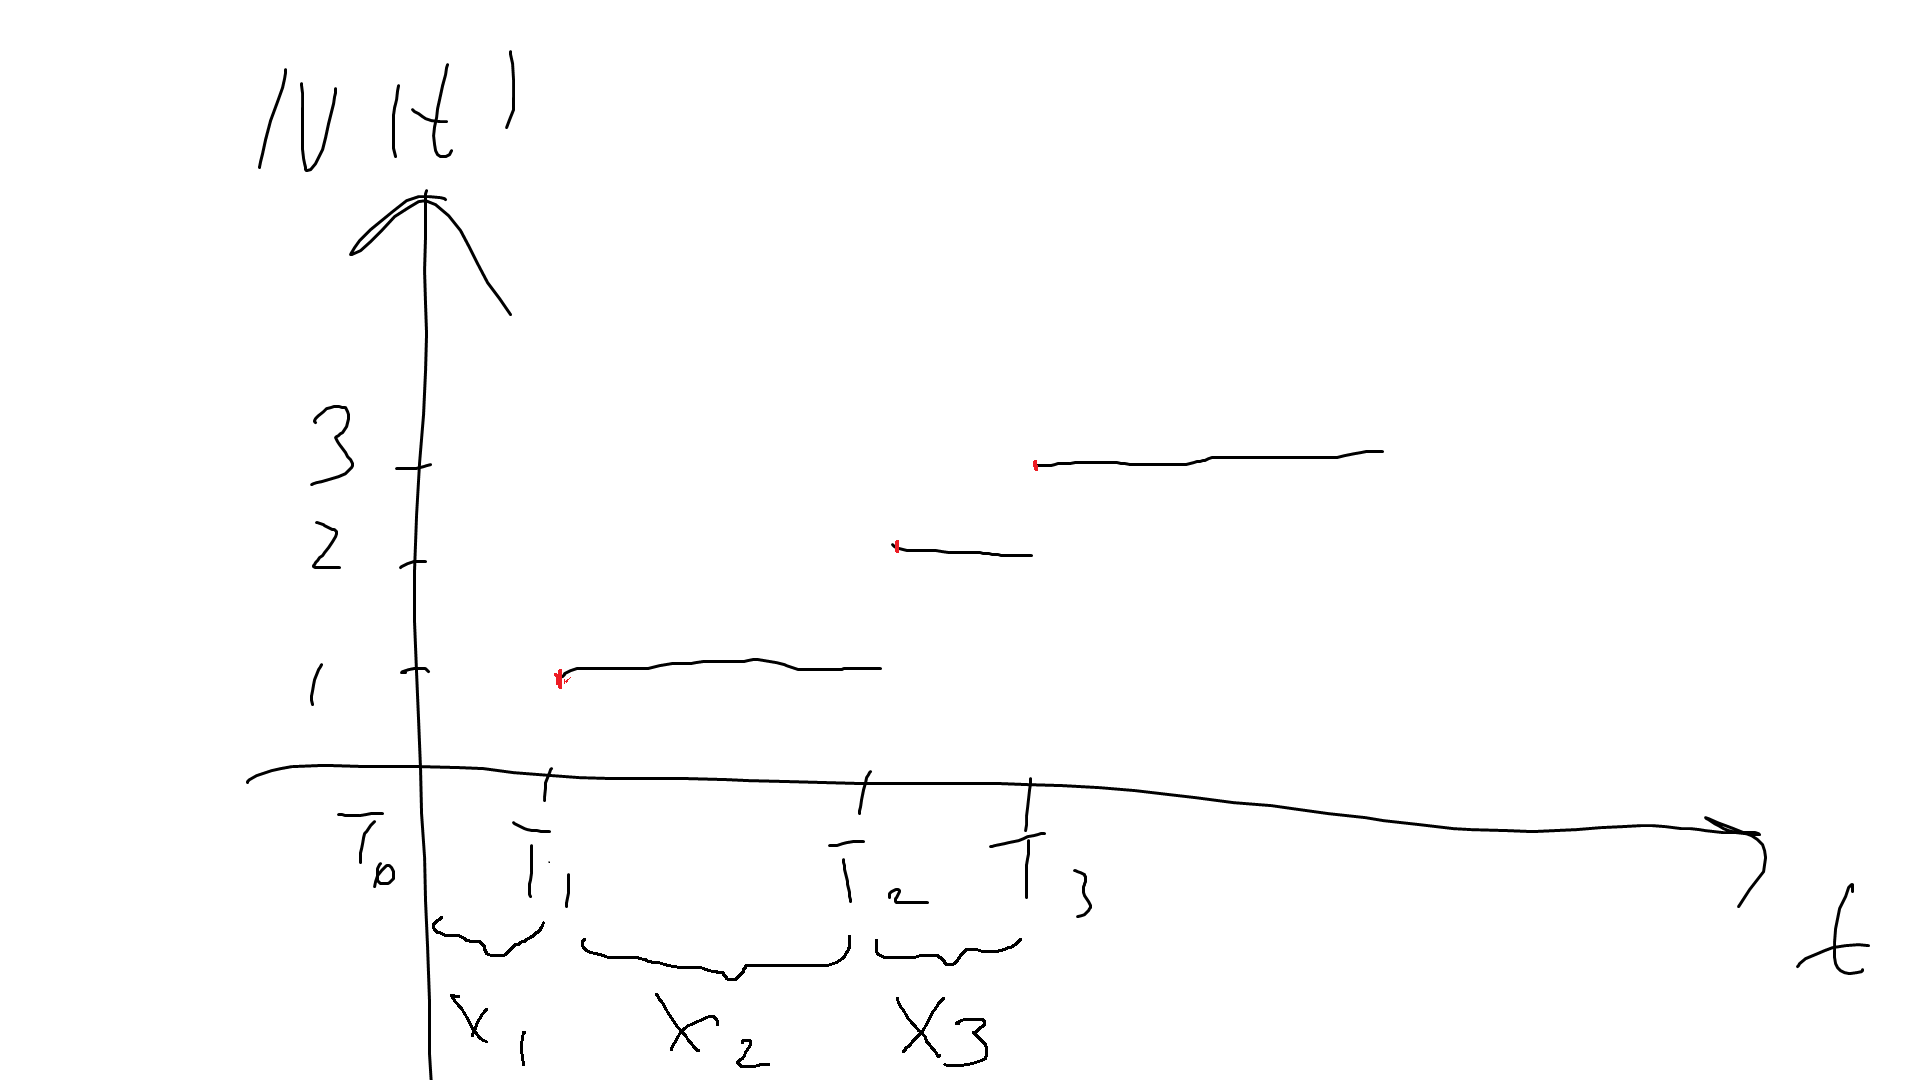
\includegraphics[scale=0.5]{image/AP_01.png}

\begin{thm}
Suppose $X_1,X_2,...$ are known. Let $T_n = \sum_1^n x_i$, note $N(t) = \max\{n:T_n \leq t\}$. Then the random variables $X_1,X_2,...$ are independent and they have the exponential distribution with parameter $\lambda$ ($Exp(\lambda)$).
\begin{proof}
\begin{equation*}
\begin{aligned}
\P(X_1 > t) = \P(N(t) = 0) = e^{-\lambda t}
\end{aligned}
\end{equation*}
So $X_1$ has $Exp(\lambda)$ distribution. Now consider $\P(X_2>t|X_1=t_1)$. This doesn't look to make much sense as $X_1$ has a continuous distribution so $\P(X_1=t_1) = 0$; however we could could consider the conditional densiy as $f_{X|Y} (x|y) =\frac{f_{X,Y}(x,y)}{f_Y(y)}$. Then $\P(X_2>t|X_1=t_1) = \P($ no arrivals in $(t_1,t_1+t)|X_1=t_1) = \P($ no arrivals in $(t_1,t_1+t)$ by independence. This is then equal to $\P($ no arrivals in $(0,t)) = \P(N(t)=0) = e^{-\lambda t}$. Then continue by induction.
\end{proof}
\end{thm}

\begin{prop} (properties of a poisson process $N$)\\
(a) $N$ has stationary independent increments, i.e.:\\
(i) If $0<t_1<...<t_n$, then $N(t_1),N(t_2)-N(t_1),...,N(t_n)-N(t_{n-1})$ are independent;\\
(ii) $N(s+t)-N(s) \xrightarrow{d} N(t)-N(0)$.\\
Amongst processes which are right continuous, non-decreasing, has only jump discontinuities of size 1, (i) and (ii) are characteristics of the Poisson process, meaning that Poisson process is the only process that has those two properties.\\
(b) Thinning:\\
Suppose insects arrive as a poisson process with parameter $\lambda$. Each insect is a mosquito with probability $\alpha$, or a skeet with probability $1-\alpha$, and the occurences of the two insects are independent. Then\\
(i) the mosquito-arrival process $F$ is a $PP(\alpha\lambda)$, 
(ii) the skeet-arrival process is $S$ a $PP((1-\alpha)\lambda)$, and 
(iii) these processes are independent.
\begin{proof}
(i) and (ii) are immediate by infinitestimal definition of a poisson process. For (iii), by independence we mean that $\P(F(t_1)=f_1,S(t_1)=s_1,...,F(t_n)=f_n,S(t_n)=s_n) = \P(F(t_1)=f_1,...,F(t_n)=f_n) \P(S(t_1)=s_1,...,S(t_n)=s_n)$ $\forall t_1,...,t_n,f_1,...,f_n,s_1,...,s_n)$.

The simple case is 
\begin{equation*}
\begin{aligned}
\P(F(t) = f, S(t) = s) &= \frac{(\lambda t)^{f+s} e^{-\lambda t}}{(f+s)!}{{f+s} \choose f} \alpha^f (1-\alpha)^s\\
&= \frac{(\alpha\lambda t)^f}{f!} e^{-\alpha\lambda t} \frac{((1-\alpha) \lambda t)^s}{s!} e^{-(1-\alpha)\lambda t}\\
&= \P(F(t) = f) \P(S(t) = s)
\end{aligned}
\end{equation*}
\end{proof}
(c) Superposition:\\
$F$: Flies arrive as $PP(\lambda_1)$;\\
$S$: Skeets arrive as $PP(\lambda_2)$, and these processes are independent. Then $N=F+S$ is a $PP(\lambda_1+\lambda_2)$. This follows by infinitesimal construction of $PP$.\\
(d) Given $N(t) = n$, write $\mathbf{T} = (T_1,...,T_n)$, $\mathbf{t} = (t_1,...,t_n)$, we have $f_{\mathbf{T}}(\mathbf{t} | N(t) = n) =\left(\frac{1}{t}\right)^n n! L(\mathbf{t})$, where $L(\mathbf{t})=1$ iff $t_1<t_2<...<t_n$.
\begin{proof}
Next time.
\end{proof}
\end{prop}

Let's complete the proof left last lecture.

\begin{thm}
Conditional on $\{N(t) = n\}$, the times $T_1,...,T_n$ have joint pdf
\begin{equation*}
\begin{aligned}
f_{ \mathbf{T} |N(t) = n} (\mathbf{t}) = \frac{n!}{t^n} L(\mathbf{t}) 1_{\{t_n \leq t\}}
\end{aligned}
\end{equation*}
where $L(\mathbf{t}) = 1_{\{t_1 \leq t_2 \leq ... \leq t_n\}}$.
\begin{proof}
The interarrival times $X_1,X_2,...,X_n$ have joint pdf
\begin{equation*}
\begin{aligned}
f_\mathbf{X}(\mathbf{x}) = \lambda^n \exp(-\lambda \sum_i^n x_i)
\end{aligned}
\end{equation*}
by change of variables, we now have (noting $T_i = X_1+...+X_i$)
\begin{equation*}
\begin{aligned}
f_\mathbf{T} (\mathbf{t}) = \lambda^n e^{-\lambda t_n} L(\mathbf{t})
\end{aligned}
\end{equation*}
Now for $C \subseteq \R^n$, we have
\begin{equation*}
\begin{aligned}
\P(T \in C | N(t) = n) &= \frac{\P(T \subseteq C, N(t) = n)}{\P(N(t) = n)}\\
&= \frac{1}{\P(N(t)=n)} \int_C \P(N(t)\\
&= n | \mathbf{T} = \mathbf{t} ) f_\mathbf{T} (\mathbf{t}) d \mathbf{t}\\
&= \frac{1}{\P(N(t) = n)} \int_{t_n \leq t} e^{-\lambda (t-t_n)}\lambda^n e^{-\lambda t_n} L(\mathbf{t}) d\mathbf{t}
\end{aligned}
\end{equation*}
the last equation is because we need ther to be no arrival between $t$ and $t_n$. Now the conditional pdf of $\mathbf{T}$ given $N(t) = n$ is
\begin{equation*}
\begin{aligned}
\frac{1}{(\lambda t)^n e^{-\lambda t} / n!} e^{-\lambda (t-t_n)} \lambda^n e^{-\lambda t_n} L(\mathbf{t}) = \frac{n! L(\mathbf{t})}{t^n} 1_{\{t_n \leq t\}}
\end{aligned}
\end{equation*}
I think somewhere in this proof we used $\P(X \in C) = \int_C g(u) du \iff f_X(u) = g(u)$, otherwise the lecture wouldn't have written this down on a separate board.
\end{proof}
\end{thm}

\newpage

\section{Continuous-time Markov chains}

This is actually quite a complicated topic, so we are going to make a lot of assumptions to simplify it.

Assume state space $S$ is countable, and we often take $S \subseteq \Z = \{ ...,-1,0,1,...\}$ (sometimes useful to assume $|S|<\infty$).

\begin{defi}
A process $X = \{X(t) : t \geq 0\}$ taking values in $S$ satisfies the \emph{Markov property} if:\\
\begin{equation*}
\begin{aligned}
\P(X(t_n) = j| X(t_1) &= i_1,...,X(t_{n-1}) = i_{n-1}) \\
&= \P(X(t_n) = j| X(t_{n-1}) = i_{n-1})
\end{aligned}
\end{equation*}
for all $i_1,i_2,...,i_{n-1}, j \in S, t_1< t_2 < ... < t_n$.

We have the transition probabilities $p_{i,j}(s,t) = \P(X(t) = j| X(s) = i)$. We, however, assume the process is homogeneous, i.e. $$p_{i,j}(s,t) = p_{i,j} (0,t-s) := p_{i,j}(t-s) \forall s,t,i,j$$so the transition probabilities only depend on the duration of time passed instead of the absolute time. We can then write this as a transition matrix $(p_{i,j}(t))_{i,j \in S}=P_t$.
\end{defi}

\begin{prop}
The family $\{P_t: t \geq 0\}$ satisfies\\
(a) $P_0 = I$;\\
(b) $P_t$ is a \emph{stochastic} matrix, i.e. a non-negative matrix with row sum 1;\\
(c) $P_{s+t} = P_s P_t$ for $s,t \geq 0$.
\begin{proof} (of (c))\\
$p_{i,j}(s+t) = \sum_{k \in S} p_{i,k}(s)p_{j,k}(t)$ by Markov Property which is just the component form of $P_{s+t} = P_s P_t$.\\
$P_{s+t} = P_s P_t$ is sometimes called the \emph{semigroup property} ($s,t \geq 0$).\\
$(P_t:t \geq 0)$ is called a \emph{stochastic semigroup}.
\end{proof}
\end{prop}

General theory involves conditions of regularity.

We assume $X$ is a right-continuous jump process.

Holding times for general chains:

Assume $X(t_0) = i$.\\
Let $H=\inf\{t>t_0:X(t) \neq i\}$. We have $$\P(H>u+v|H>u) = \P(H>v) \ (*)$$ by Markov Property ($u,v \geq 0$).\\
Let $G(u) = \P(H>u)$. By (*), we get $\frac{G(u+v)}{G(u)} = G(v)$, so $G(u+v) = G(u)G(v)$.\\
We know $G(0) = 1$, and $G$ is non-increasing.\\
Solution: $G(n) = G(1)G(n-1) = G(1)^n$ $\forall n \in \N$. Also $G(p/q)... G(p/q) =G(p) = G(1)^p$ so $G(p/q) = G(1)^{p/q}$, hence $G(u) = G(1)^u$ for $u \geq 0$. We deduce that $G(u) = e^{-\alpha u}$ for some $\alpha>0$.

\begin{lemma}
A random variable $X>0$ has an exponential distribution iff it has the \emph{lack of memory property}: $\P(X>u+v|X>u) = \P(X>v)$ $\forall u,v > 0$.
\end{lemma}

A MC s a combination of exponential-distribution holding times, and a transition matrix for the \emph{jump chain} $Y=(Y_n)$ given by $Y_0 =X(0)$, $Y_1 = X(T_1)$, where $T_1 = \inf\{t:X(t) \neq X(0)\}$, and $Y_n = X(T_n)$ where $T_{n+1} = \inf \{t > T_n: X(t) \neq X(T_n)\}$. $Y$ is a \emph{discrete-time Markov chain.}

If in state $i$, want $H$, we jump to state $j\neq i$ with probability $\frac{g_{ij}}{\alpha_i}$. Intensity of a jump is $\alpha_i$, and intensity of a jump to state $j$ is $g_{ij}$.\\
Note a transition from $i$ to itself is not deemed to be a transition.

We have $p_{ij} (h) = g_{ij} h + o(j)$ ($j \neq i$), $p_{ij}(h) = 1- \sum_{j \neq i} p_{ij}(h) = 1-h\sum_{j \neq i} g_{ij} + o(h) = 1-\alpha_i h + o(h) = 1+g_{ii} h + o(h)$, where we let $g_{ii} = -\alpha_i$. Now we let $G$ be the matrix $(g_{ij})$, with the off-diagonal terms the previous $g_{ij}$'s, but the diagonal terms $g_{ii}$ as defined just now (so as to make row sums 0). Now the off-diagonal terms are non-negative, and diagonal terms are non-positive. We call $G$ the \emph{generator} of the chain (otherwise known as the $Q$-matrix).

Conclusion: $\frac{P_t - I}{t} \xrightarrow{t \to 0^+} G$.\\
Questions of regularity: OK if $|S| < \infty$.

(?)
\begin{equation*}
\begin{aligned}
p_{ij}(t+h) &= \sum_k p_{ik}(t) p_{kj}(h)\\
&= \sum_{k \neq j} p_{ik}(t) [g_{kj} h + o(h) + p_{ij}(t) (1+g_{jj} h + o(h))\\
&= \sum_k p_{ik} (t) g_{kj}\\
&= P_t \cdot G
\end{aligned}
\end{equation*}
this is the (Kolmogov) Forward Equation.

$p_{ij}(t+h) = \sum_k p_{ik}(h) p_{kj}(t)$, so $P't = GP_t$, called the K-Backward equation.

Interchange of limits requires justification -- it's OK if $|S| < \infty$.

Now $P'_t = P_t G$, we can rewrite this as $f'=fg$, which gives $f(t) = A e^{gt}$. So the solution should be $P_t = P_0(=I)e^{tG}$ (i.e. $=\sum_{k=0}^\infty \frac{t^k}{k!} G^k$).

In many cases, the solution to the forward and/or backward equation is the function $P=e^{tG}$.

A mistake has been made! The definition for holding time is wrong. It should be $H=\inf\{ t-t_0: X(t) \neq X(t_0), t > t_0\}$ (the length rather than the absolute time).

Let's look at an example now.
\begin{eg}
Let $S=\{1,2\}$, $G={{-\alpha \ \alpha} \choose {\beta \ -\beta}}$, where $\alpha\beta > 0$. What are the $p_{ij}(t)$?\\
There are only two states, so let's find
\begin{equation*}
\begin{aligned}
p_{11}'(t) = -\alpha p_{11} + \beta p_{12},\\
p_{12}'(t) = \alpha p_{11}(t) - \beta p_{12}(t)\\
...
\end{aligned}
\end{equation*}
So we get a bunch of differential equations, with boundary conditions $p_{11}(0) = p_{22}(0) =1$. This has a unique solution (check). We get $P_t = e^{tG} =\sum_n \frac{t^n}{n!} A \Lambda^n A^{-1}$ wher we diagonalize $G=A\Lambda A^{-1}$. But $e^{t\Lambda}$ is equal to $Diag(e^{\lambda_1 t}, e^{\lambda_2 t} ...)$. Each $p_{ij}(t)$ has the form $\sum_k e^{\lambda_k t} c_K (i,j)$, where we need to find the constants $c_k(i,j)$.
\end{eg}

\begin{lemma}
Let $i,s \in S$. Then either $p_{ij}(t)=0$ $\forall t>0$, or $p_{ij}(t) > 0$ $\forall t > 0$ (this is because our time here is continuous; we can fit in any number of jumps in any time length with positive probability).
\begin{proof}
Assume $p_{ij}(T) > 0$ for some $T>0$. Then for $t>T$, $p_{ij}(t) \geq p_{ij}(T) \P_j (X_j > t-T) > 0$ (start in $j$ and holding time $> t-T$, which is positive).\\
For $t<T$: there exists finite sequence of jumps from $i$ to $j$ in time $T$, so there exists $i_1,i_2,...,i_n \in S$ with $g_{i,i_1}g_{i_1,i_2}...g_{i_n,j}>0$, where $g_{i,j}$ is as defined previously. Then we can just divide the time $(0,t)$ into $n+1$ intervals. Then $p_{i,j}(t) \geq p_{i,i_1}(t/(n+1))...p_{t_n,j}(t/(n+1)) > 0$ (this is an applied course, so we don't care that much).
\end{proof}
\end{lemma}

\begin{defi}
The chain $X$ on state space is \emph{irreducible} if $\forall i,j \in S$, $\forall t > 0, p_{i,j}(t)>0$ ($\iff \exists t>0, p_{i,j}(t)>0$).
\end{defi}

A distribution $\pi$ on $S$ is invariant (or stationary, or equilibrium distribution) if $\pi = \pi P_t$ for all $t \geq 0$.

Note: if $X(0)$ has distribution $\mu_0$, then $X(t)$ has distribution $\mu_t = \mu_0 P_t$ ($\mu_t(j) = \sum_i \mu_0(i) p_{i,j}(t)$).

Note: (a) Differentiate $\pi = \pi P_t$ to get $0 = \pi G$;\\
(b) If $P_t = e^{tG}$ then $\pi G = 0$ iff $\pi G^n = 0$ for $n \geq 1$ iff $\pi \sum_n \frac{t^n}{n!} G^n = \pi$ iff $\pi P_t = \pi$.

\begin{thm}
Let $X$ be irreducible. If there exist an invariant distribution $\pi$, then it is unique (what a surpise), and $p_{ij}(t) \to \pi_j$ as $t\to \infty$. Can we prove this in the remaining 11 minutes? Let's try:
\begin{proof}
Let $h>0$. Then $Y_n=X(nh)$. So $Y$ is a 'skeleton' of $X$. $Y$ is a markov chain. Since $X$ is irreducible, so is $Y$. $Y$ has invariant distribution $\pi$, hence $\pi$ is unique. (?) Since $X$ is irreducible, $Y$ is aperiodic(?). Hence $p_{ij}(nh) \to \pi_{ij}$ as $n \to \infty$. Since this holds for all $h \in \Q^+$, we deduce that $p_{ij}(t) \to \pi_j$ as $t\to \infty$ through the rationals. The conclusion follows by continuity of $p_{ij}(\cdot)$.
\end{proof}
\end{thm}

\begin{lemma}
The functions $p_{ij}(\cdot)$ are continuous.
\end{lemma}

Last time we claimed that if $\forall h>0$, $p_{ij}(nh) \pi_j$ as $n \to \infty$, then $p_{ij}(t) \to \pi_j$ as $t \to \infty$. However this is wrong as the rate of convergence might depend on $h$.\\
From some theorem in Linear Analysis it is known that if $p$ is continuous then the above is actually true. But this is an applied course so let's not assume Linear Analysis. Let's now prove it with the following lemma:
\begin{lemma}
$p_{ij}(\cdot)$ is uniformly continuous in $t$.
\begin{proof}
\begin{equation*}
\begin{aligned}
|p_{ij}(t+h)-p_{ij}(t)| &= |[\sum_k p_{ik}(h) p_{kj}(t)] - p_{ij}(t)|\\
&\leq |\sum_{k \neq i} p_{ik}(h) p_{kj}(t) | + |p_{ij}(t) [1- p_{ii}(h)]|\\
&\leq [1-p_{ii}(h)]\\
&\leq 2(1-e^{-g_i h}) \to 0
\end{aligned}
\end{equation*}
as $h \to 0$.
\end{proof}
\end{lemma}
Back to the theorem: let $t>0$, $\exists h$ s.t. $|p_{ij}(t+h) - p_{ij}(t)| < \frac{1}{2}\varepsilon \forall t$. Then $|p_{ij}(t) - p_{ij}(\lfloor t/h \rfloor h)| < \frac{1}{2} \varepsilon$. Pick $N$ s.t. $|p_{ij}(nh) -\pi_j| < \varepsilon/2$ for $n \geq N$. For $t>(n+1)h$ we have $|p_{ij}(t) - \pi_j| \leq |p_{ij}(t) - p_{ij}(\lfloor t/h\rfloor h)| + |p_{ij}(\lfloor t/h \rfloor h) - \pi_j) \leq \frac{1}{2}\varepsilon + \frac{1}{2} \varepsilon$ so done.

\emph{Explosion}:\\
Let $S$ be countable. $H=(h_{i,j}:i,j \in S)$ is the transition matrix of a discrete time markov chain $Z = (Z_n : n \geq 0)$ on $S$. Assume $h_{i,i} = 0 \forall i \in S$. Let $(g_i:i \in S)$ be non-negative reals. Inifinitesimal definition of $X$: $g_{ij} = g_i h_{ij}$ if $i \neq j$, and $-g_i$ if $i=j$. Holding time definition: $X(0) = Z_0$. Given $Z$, let $U_0,U_1,...$ be independent exponential random variables, where $U_n$ has parameter $g_{Z_n}$.

We define $T_n = U_0 + ... + U_{n-1}$, the time of the $n^{th}$ jump. $X(t) = Z_n$ if $T_n \leq t < T_{n+1}$.

$T_n \to T_\infty = \sum_0^\infty U_n$. Say the process [explodes if $T_\infty < \infty]$, or explodes if $\P(T_\infty < \infty) > 0$.

We augment the state space $S$ to $S' = S \cup \{\infty\}$ (cemetery state, means $\infty$ is absorbing). Assume: at $T_\infty$, the chain enters the cemetery state labelled $\infty$. Such a process is called minimal.

\begin{thm}
The process $X$, constructed via holding times as above, does not explode if any of the following occurs:\\
(a) $|S| < \infty$;\\
(b) $\sup_i g_i < \infty$;\\
(c) $X(0) = i$, where $i$ is recurrent for the jump chain $Z$.
\end{thm}

\begin{lemma}
Let $X_1,...$ be independent random variales, and $X_i$ has distribution $Exp(\lambda_{i-1})$. Let $T_\infty = \sum_1^\infty X_i$. $\P(T_\infty < \infty = 0$ if $\sum \lambda_i^{-1} = \infty$, and 1 otherwise.
\begin{proof}
\begin{equation*}
\begin{aligned}
\E(T_\infty) &= \E(\sum_1^\infty X_i)\\
&= \E (\lim_{N \to \infty} \sum_1^N X_i)\\
&= \lim_{N \to \infty} \E(\sum_1^N X_i)\\
&= \lim_{N \to \infty} \sum_1^N \frac{1}{\lambda_{i-1}}\\
&= \sum_1^\infty \frac{1}{\lambda_{i-1}}
\end{aligned}
\end{equation*}
Now If $\sum \frac{1}{\lambda_{i-1}} < \infty$, then $\E(T_\infty) < \infty$. So $\P(T_\infty = \infty) = 0$.\\
The other part will be proven in next lecture.\\
Problem sheet 2 is online!\\
For the other part we have 
\begin{equation*}
\begin{aligned}
\E(e^{-T_\infty}) &= \E(\prod_1^\infty e^{-X_i})\\
&= \prod_1^\infty \E(e^{-X_i})\\
&= \prod_1^\infty \frac{1}{1+\lambda_i^{-1}} = 0
\end{aligned}
\end{equation*}
the second equation by dominated convergence. So $\P(e^{-T_\infty} = 0) = 1$.
\end{proof}
\end{lemma}

Proof of theorem:
\begin{proof}
(a) to (b):(proved? where) \\
Proof that (b) implies no explosion:\\
Suppose $g+i \leq \gamma < \infty$ for some $\gamma$. Then $\sum_0^\infty$ is a sum of independent exponential distribution r.v.s, i.e .$U_i \sim Exp(g_{z_i})$. hence $g_{Z_i} U_i \sim Exp(1)$.\\
Now $\gamma \sum_0^\infty U_i \geq \sum_i g_{Z_i} U_i$ is sum of independent $Exp(1)$ random variables, which diverges with probability 1. So $\P(T_\infty < \infty) = 0$.\\
Proof that (c) implies no explosion: We know there are infinitely many $n$ with $Z_n = i$ (a.s.) since $i$ is recurrent. Now $T_\infty \geq$ sum of infinitely many indepnedent holding times in state $i$ = sum of independent $Exp(g_i)$ random variables which diverges a.s.. So $\P(T_\infty < \infty) = 0$.
\end{proof}

\begin{eg}
Let $Z$ be a discrete-time chain with transition matrix $H$, where $H_{i,i} = 0$ $\forall i \in S$. Let $N$ be a PP with intensity $\lambda>0$.\\
Let $X(t) = Z_n$ if $T_n \leq t < T_{n+1}$, where $T_n$ is the time of the $n^{th}$ arrival in $N$. Now
\begin{equation*}
\begin{aligned}
p_{ij}(t) &= \sum_{n=0}^\infty \P(X(t) = j | X(0)=i,N(t) = n) \P(N(t) = n)\\
&= \sum_n \frac{(\lambda t)^n}{e^{-\lambda t}}{n!} (H^n)_{i,j}
\end{aligned}
\end{equation*}
We have
\begin{equation*}
\begin{aligned}
e^{\lambda t} I = \sum_{n=0}^\infty \frac{(-\lambda t)^n}{n!} I^n = e^{-\lambda t I}
\end{aligned}
\end{equation*}
So $P_t = e^{\lambda t(H-I)^n} = e^{tG}$ where $G=\lambda(H-I)$.
\end{eg}

\begin{defi}
State $i$ of the continuous time MC $X$ is recurrent if $\P_i(\{t \geq 0: X(t) = i\}$ is unbounded$)=1$; it is transient if the above probability is 0.
\end{defi}

\begin{thm}
(a) If $g_i = 0$, then $i$ is recurrent.\\
(b) Let $g_i>0$. State $i$ is recurrent for $X$ if it is recurrent for the jump chain $Z$. Furthermore, $i$ is recurrent if 
\begin{equation*}
\begin{aligned}
\int_0^\infty p_{ii}(t) dt = \infty
\end{aligned}
\end{equation*}
\begin{proof}
(a) If $g_i = 0$ then $\{(X(t) = i, \forall t) = 1$.\\
(b) Let $g_i>0$. If $i$ is transient for $Z$, then $Z$ has a last visit to $i$ at some time $N$. So $X(t) \neq i$ for $t>T_{N+1}$. So $i$ is transient for $X$. If $i$ is recurrent for $Z$, the times at which $Z$ visits $i$ is infinite a.s.. By last theorem, there is no explosion. So the chain $\{T_n:Z_n=i\}$ is unbounded a.s.. ($T_n$ is time of $n^{th}$ jump of $X$). Hence $i$ is recurrent for $X$.
Note: the proof implies a non-recurrent state is transient.\\
Now
\begin{equation*}
\begin{aligned}
\int_0^\infty p_{ii}(t) dt &= \int_0^\infty \E_i(1_{X(t) = i}) dt\\ 
&= \E_i (\int 1_{X(t)=i} dt) \\
&= \E_i(\sum_n U_n 1_{\{Z_n=i\}})\\
&= \sum_n \frac{1}{g_i} \P_i (Z_n = i)\\
&= \frac{1}{g_i} \sum_n (H^n)_{i,i} = \infty
\end{aligned}
\end{equation*}
if $i$ is recurrent for $Z$.
\end{proof}
\end{thm}

Assume $g_j>0 \forall j$. $g_i=0$.

\newpage
\section{Birth Process}
This is a continuous-time Markov Chain with generator $g_{n,n+1} = \lambda_n$ and $g_{n,m} = 0$ for $m \neq n,n+1$. When in state $n$, we jump to $n+1$ at rate $\lambda_n$, otherwise stay at $n$. $\lambda_n$ is just a constant, so if $\lambda_n=\lambda$ $\forall_n$ then this is just a Poisson process.

For a \emph{simple birth process}, living particles give birth to single offspring at rate $\lambda$ independently of other offsprings.\\
Let $N_t =$ number of individuals alive at time $t$. Then
\begin{equation*}
\begin{aligned}
\P(N_{t+h} = n+m | N_t = n) = {n \choose m} (\lambda h+o(h))^m (1-\lambda h -o(h) )^{n-m} + o(h) = \left\{\begin{array}{ll}
1-n\lambda h + o(h) & m=0\\
n\lambda h + o(h) & m=1\\
o(h) & m \geq 2
\end{array}
\right.
\end{aligned}
\end{equation*}
Hence this is a birth process with $\lambda_n = n\lambda$.

Let's look at another example:

\begin{eg}
Simple birth with immigration: in this model we have $\lambda_n = n\lambda + \varepsilon$, where $\lambda$ is the birth rate and $\varepsilon$ is the immigration rate.

Kolmogorov equations:\\
Forward equation: condition on $N_t$, $p'_{ij}(t) = \lambda_{j-1} p_{i,j-1}(t) - \lambda_j p_{ij}(t), i,j \geq 0, t \geq 0$, so $P'_t = P_t G$.\\
Backward eqautions: condition on $N_h$, $p'_{ij}(t) = \lambda_i p_{i+1,j}(t) - \lambda_i p_{i,j}(t)$. So $P'_t = GP_t$.\\
Boundary condition: $p_{i,j}(0) = \delta_{i,j}$.\\
Facts: $p_{i,i-1}(t) = 0$.
\end{eg}

\begin{thm}
For a birth process, the forward equations have a unique solution, which satisfies the backward equation.
\begin{proof}
$j=i$ in Forward equation: $p_{ii}'(t) = -\lambda_i p_{i,i}(t)$. Hence $p_{ii}(t) = e^{-\lambda_i t}$,\\
$p_{i,i+1}'(t) = \lambda_i p_{i,i}(t) - \lambda_{i+1} p_{i,i+1}(t)$.\\
Hence $p_{i,i+1}(t)$ and hence $p_{i,j}(t)$ by induciton.
\end{proof}
\end{thm}

Laplace transforms:\\
Let $g:\R^+ \to \R$. We define the laplace transform of $g$,
\begin{equation*}
\begin{aligned}
\hat{g}(\theta) = \int_0^\infty e^{-\theta t} g(t) dt
\end{aligned}
\end{equation*}
for $\theta > 0$.

Remember we have the mgf, $E(e^{\theta x}) = \int e^{\theta t} f_x(t) dt$.

We have the Laplace inverse theorem (in Complex Methods). We know
\begin{equation*}
\begin{aligned}
\int e^{-\theta t} g'(t) dt = [e^{-\theta t} g]_0^\infty + \int \theta e^{-\theta t} g(t) dt\\
&= -g(0) + \theta \hat{g}(\theta) = \hat{g'}
\end{aligned}
\end{equation*}

Now
\begin{equation*}
\begin{aligned}
&\theta \hat{p}_{ij} - \delta_{i,j} = \lambda_{j-1} \hat{p}_{i,j-1} - \lambda_j \hat{p}_{i,j}\\
&\implies (\theta+\lambda_j) \hat{p}_{ij} = \delta_{i,j} + \lambda_{j-1} \hat{p}_{i,j-1}
\end{aligned}
\end{equation*}
hence the $\hat{p}_{i,j}$'s are
\begin{equation*}
\begin{aligned}
\hat{p}_{ij}(\theta) = \frac{1}{\lambda_j} \frac{\lambda_j}{\theta+\lambda_i} ... \frac{\lambda_j}{\theta+\lambda_j}, i \leq j.
\end{aligned}
\end{equation*}

It's easy to check that this Laplace transform satisfies the "Laplace" equation of the backward "system",
\begin{equation*}
\begin{aligned}
-\delta_{ij} + \theta \hat{p}_{ij} = \lambda \hat{p}_{i+1,j} -\lambda_j \hat{p}_{i,j}
\end{aligned}
\end{equation*}

\begin{thm}
The forward equations have a unique solution $(p_{i,j}(t))$ which is the minimal solution to the backward equation, in that, for any other solutions $(\pi_{i,j}(t))$ to the backward equation, we have
\begin{equation*}
\begin{aligned}
p_{i,j}(t) \leq \pi_{i,j}(t) \forall i,j,t
\end{aligned}
\end{equation*}
The lecture thinks the proof might be in a book of Norris, or online notes by Burostychi + Sousi(?).
\end{thm}

If we know in addition that $\sum_j p_{i,j}(t) = 1$ $\forall i$, then we know $p_{i,j}(t)$ is the unique solution to the backward equation, as any other solution $\pi_{i,j}(t)$ would have a sum exceeding 1.

Assume we have a MC $X=(X(t))$, and jump chain $Y=(Y_n)$. Assume $g_j>0$ $\forall j$. Speaking (probably not this word) $X$ via holding time definition. Assume $X$ is a minimal process. We can define the transition probability: 
\begin{equation*}
\begin{aligned}
p_{i,j}(t) = \P_i(X(t)=j) \forall i,j \in S
\end{aligned}
\end{equation*}
The $(p_{i,j}(t))$ satify the C-K equations.

Something we've talked about in the last lecture:

(a) $(p_{i,j}(t))=P_t$ is the minimal no-negative solution to forward equation $P_t' = P_tG$, $P_0 = I$. Here minimal: for any non-negative solution $\pi$ we have $p_{i,j}(t) \leq \pi_{i,j}(t)$ $\forall i,j,t$;\\
a
(b) $P_r$ is the minimal non-negative solution to the backward equation $P'_t=GP_t$, $P_0=I$.

\subsection{Strong Markov Property}
A \emph{Stopping time} is a random variable $T$ taking values in $[0,\infty) \cup \{\infty\}$ such that $\{T \leq t\} \in \mathcal{F}_T = \sigma(\{X(s):s\leq t\})$, the smallest $\sigma$-algebra on which every $X(s)$ for $s\leq t$ is measurable.

Strong Markov Property: Let $X$ be a MC, with given generator and initial distribution. Let $T$ be a stopping time for $X$. Given $T<S$, and $X(T) = i$. Then $\{X(T+t):t \geq 0\}$ is a MP with generator $G$ and initial state $X(T) =i$, which is independent of $\{X(s):s \leq T\}$.\\
The proof is omitted for measure-theoretic reasons.

Hitting times: Let $X$ be a MC, as usual, with generator $G$. Hitting time of $A \subseteq S$ is $T_A = \inf \{t \geq 0: X(t) \in A\}$.

Note: $T_A$ is a stopping time. The jump chain $Y$ has hitting time $H_A= \inf\{n \geq 0:Y_n \in A\}$. Now $\{T_A < \infty\} = \{H_A < \infty\}$. We call $h_A(i) = \P_i(T_A < \infty)$ (starting in $i$). Then $h_A(i) = \P_i(H_A < \infty)$. Hence $h_A$ is least non-negative solution to $h_A(i) = 1$ if $i \in A$, $h_A (i) = \sum_{j \in S} \frac{g_{i,j}}{g_i} h_A(j)$ if $i \not\in A$\\
i.e. $h_A$ satisfies the equations, and $h+A(i) \leq h'_A(i)$ $\forall i$ for any other non-zero solution $h'_A$.

$-g_{i,i}h_A(i) = \sum_{j \neq i} g_{i,j} h_A(j)$, i.e. $Gh_A = 0$.

Hence $h_A$ is the least non-negative solution to:\\
$h_A(i) = 1$ if $i \in A$,\\
$Gh_A(i) = 0$ if $i \not\in A$.

Let $k_A(i) = \E_i(T_A)$, and assume $h_A(i) = 1$ $\forall i$. $k_A(i) = 0$ if $i \in A$. Let $i \not\in A$. Then $k_A(i) = \frac{1}{g_i} + \sum_{j \neq i} \frac{g_{i,j}}{g_i} k_A(j)$. By SMP, $-g_{ii}k_A(i) = 1+\sum_{j \neq i} g_{ij} k_A(j)$, so $Gk_A(i) = -1$ for $i \not\in A$.

\begin{thm}
$k_A$ is minimal non-negative solution to $k_A(i) = 0$ if $i\in A$ and $Gk_A(i) = -1$ if $i \not\in A$.
\end{thm}

\iffalse
\begin{equation*}
\begin{aligned}

\end{aligned}
\end{equation*}
\fi
\end{document}
